\documentclass[11pt]{article}
\usepackage[a4paper,top=1.5cm,bottom=3.0cm,left=1.9cm,right=1.9cm,footskip=2.0cm]{geometry}
\usepackage{graphicx}
\usepackage[table]{xcolor}
\usepackage{ragged2e}
\usepackage{fancyhdr}
\usepackage{fontspec}
\setmainfont{Noto Sans Tamil}
\setsansfont{Noto Sans Tamil}
\newfontfamily\latinfont{Carlito}
\renewcommand{\familydefault}{\sfdefault}
\definecolor{titleblue}{HTML}{0F2F4A}
\definecolor{textblack}{HTML}{1A1A1A}
\definecolor{rule}{HTML}{C9C4C0}
\definecolor{muted}{HTML}{6B635E}
\setlength{\parindent}{0pt}\setlength{\parskip}{0.5em}

\setlength{\headheight}{0pt}\setlength{\headsep}{0pt}
\pagestyle{fancy}
\fancyhf{}
\renewcommand{\headrulewidth}{0pt}
\renewcommand{\footrulewidth}{0pt}
\fancyfoot[C]{%
  \begin{minipage}{\textwidth}
    {\color{rule}\hrule height 0.7pt}\vspace{4pt}
    \noindent
    \begin{minipage}[c]{0.66\textwidth}{\scriptsize\color{muted}{\latinfont Developed by the Water and Climate Lab, IIT Gandhinagar, using hydro-meteorological data from IMD and partner agencies}.}\end{minipage}\hfill
    \begin{minipage}[c]{0.32\textwidth}\raggedleft
      
\includegraphics[height=0.62cm]{wcl.png}\hspace{6pt}%
      
\includegraphics[height=0.62cm]{iitgn.png}\hspace{6pt}%
      
\includegraphics[height=0.62cm]{imd.png}
    \end{minipage}\\[3pt]
    {\scriptsize\color{muted}© {\latinfont 2026 Water and Climate Lab} · {\latinfont Indian Institute of Technology Gandhinagar} · {\latinfont For research and demonstration purposes}.}
  \end{minipage}%
}

\begin{document}

\noindent
\begin{minipage}[c]{0.16\textwidth}
\includegraphics[width=\linewidth]{wcl.png}\end{minipage}\hfill
\begin{minipage}[c]{0.80\textwidth}\raggedleft
  {\fontsize{19}{22}\selectfont\bfseries\color{titleblue}{\latinfont National Drought Summary}}\\[2pt]
  {\normalsize\color{muted}{\latinfont Week ending May 20, 2026}}
\end{minipage}
\vspace{6pt}{\color{rule}\hrule height 1pt}\vspace{10pt}
\begin{center}
  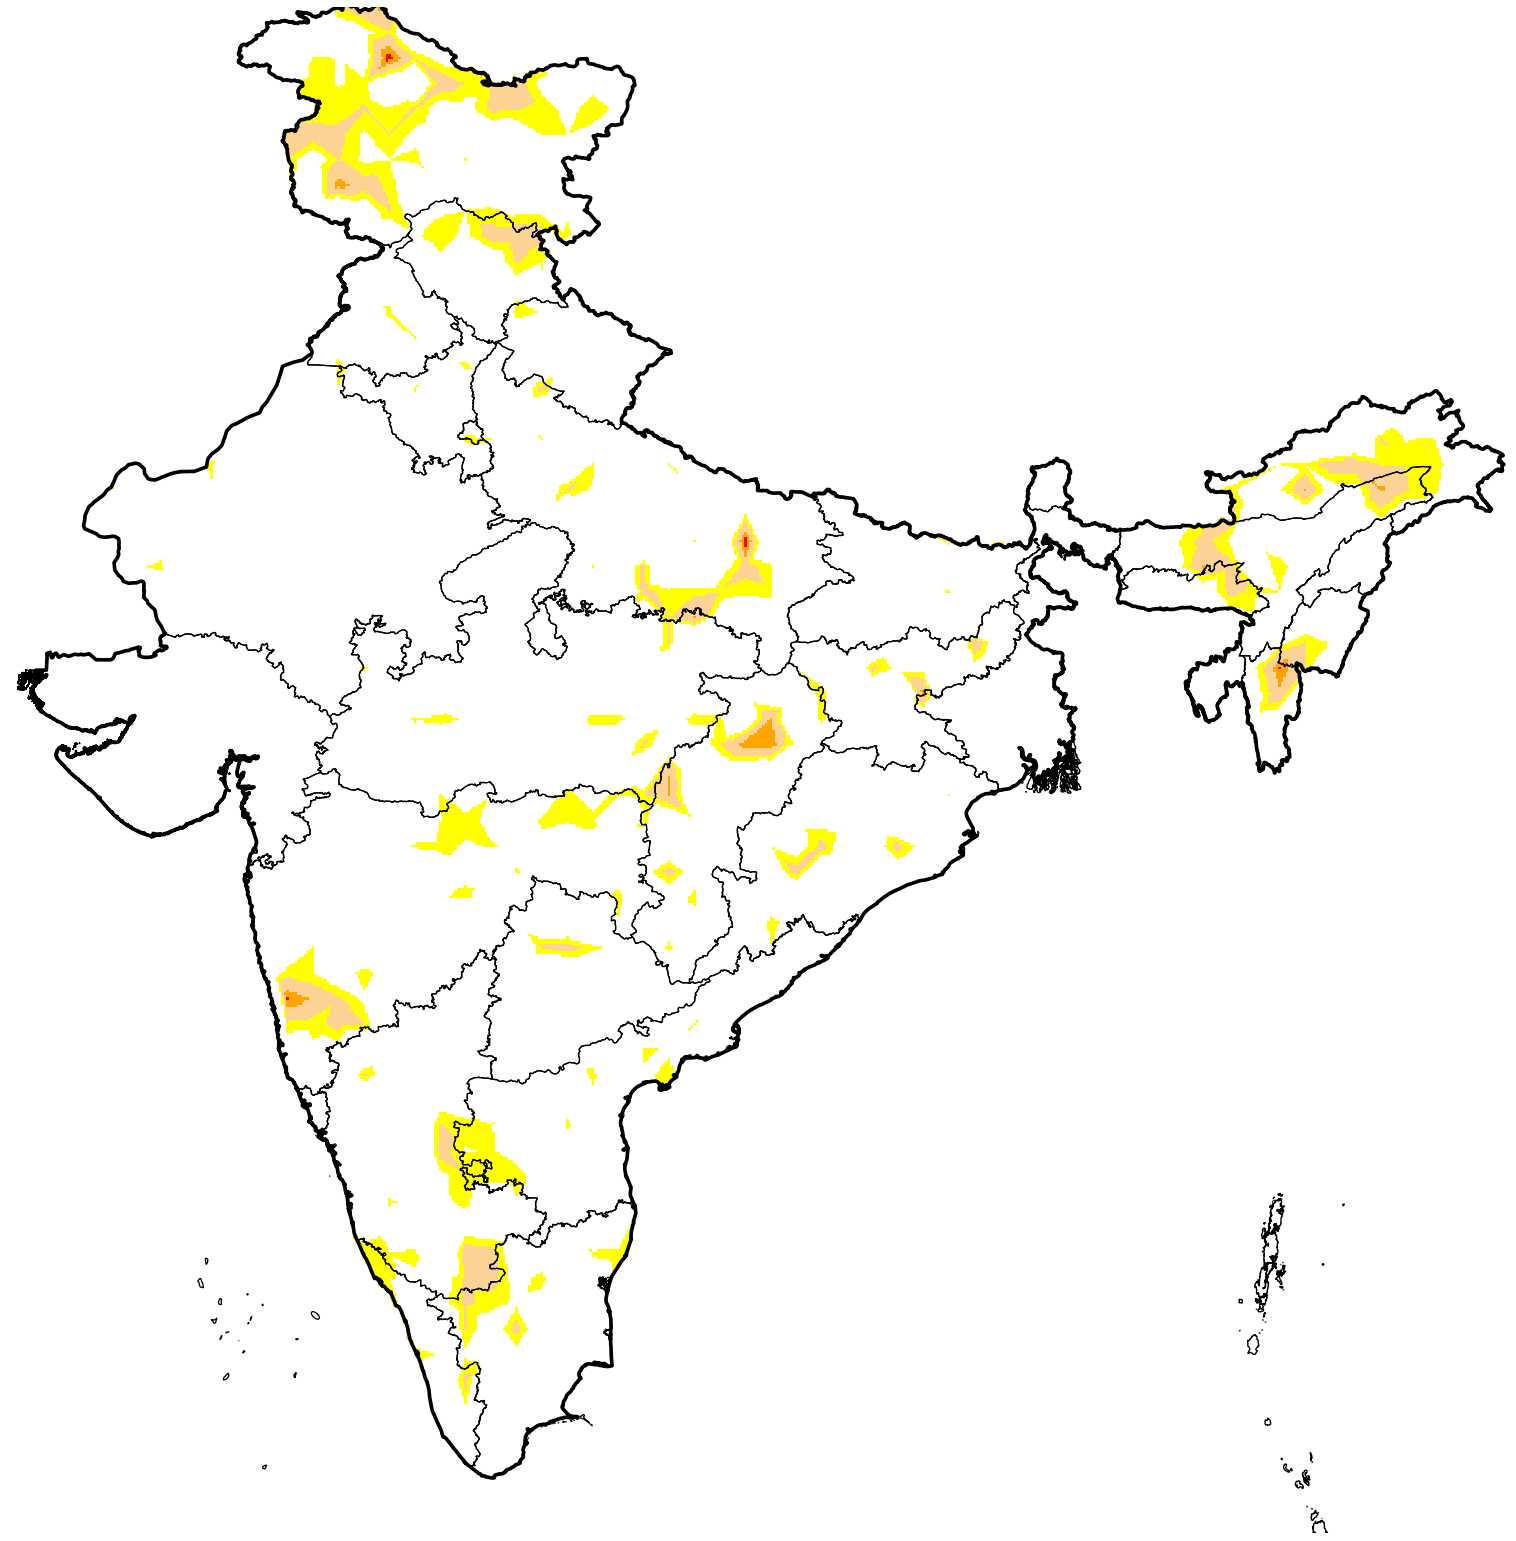
\includegraphics[width=0.60\textwidth]{cdi_map.png}\\[3pt]
  {\small\color{muted}{\latinfont Combined Drought Index (CDI) for the week ending May 20, 2026}.}
\end{center}
\vspace{2pt}
{\large\bfseries\color{titleblue}{\latinfont Summary}}\\[3pt]
{\justifying\normalsize\color{textblack}இந்த வார தேசிய வறட்சி நிலைமை பெரும்பாலான இந்தியா சாதாரண பிரிவில் உள்ளது, இதில் {\latinfont 84.7} சதவீதம் பகுதி சாதாரண என வகைப்படுத்தப்பட்டுள்ளது. இந்த வாரம் வறட்சி நிலைமைகளை அனுபவித்த மொத்த பகுதி, குறிப்பாக {\latinfont D0} மற்றும் அதற்கு மேல், {\latinfont 15.3}\% ஆகும். இந்த புள்ளி முந்தைய காலங்களுடன் ஒப்பிடும்போது வறட்சிப் பகுதியில் ஒரு சுருக்கத்தைக் பிரதிபலிக்கிறது, ஏனெனில் மொத்த வறட்சிப் பகுதி வாரந்தோறும் {\latinfont 0.9} சதவீத புள்ளிகள் குறைந்து, கடந்த வாரத்தில் {\latinfont 16.2}\% இலிருந்து தற்போது {\latinfont 15.3}\% ஆகக் குறைந்துள்ளது. வறட்சியால் அதிகம் பாதிக்கப்பட்டுள்ள பகுதிகள் டெல்லியின் {\latinfont NCT} ஆகும், அதன் {\latinfont 52.2} சதவீதம் பகுதி வறட்சியில் உள்ளது, அதைத் தொடர்ந்து மணிப்பூர் {\latinfont 42.3}\%, மிசோரம் {\latinfont 40.8}\%, அருணாச்சல பிரதேசம் {\latinfont 40.3}\%, ஜம்மு காஷ்மீர் {\latinfont 38.9}\% மற்றும் மேகாலயா {\latinfont 34.1}\% ஆகும். இதற்கு நேர்மாறாக, மேற்கு வங்காளம் அதன் பகுதியின் {\latinfont 0.0}\% வறட்சியில் புகாரளித்தது, அதே நேரத்தில் ராஜஸ்தான் வறட்சியால் மிகக் குறைவாகப் பாதிக்கப்பட்ட மாநிலமாக அதன் பகுதியின் {\latinfont 1.0}\% வறட்சியில் உள்ளது.\par}
\vspace{8pt}
{\large\bfseries\color{titleblue}{\latinfont Regional Outlook}}\\[2pt]
{\normalsize\color{titleblue}\textbf{{\latinfont North}}}\enspace {\normalsize\color{textblack}{\latinfont Moderate, scattered drought. About 28}\% {\latinfont of the area is in drought (D0}–{\latinfont D4)}.} \par\smallskip {\normalsize\color{titleblue}\textbf{{\latinfont Northwest}}}\enspace {\normalsize\color{textblack}{\latinfont Largely normal conditions. About 4}\% {\latinfont of the area is in drought (D0}–{\latinfont D4)}.} \par\smallskip {\normalsize\color{titleblue}\textbf{{\latinfont Northeast}}}\enspace {\normalsize\color{textblack}{\latinfont Moderate, scattered drought. About 27}\% {\latinfont of the area is in drought (D0}–{\latinfont D4). Pockets of severe-or-worse conditions are present}.} \par\smallskip {\normalsize\color{titleblue}\textbf{{\latinfont East}}}\enspace {\normalsize\color{textblack}{\latinfont Mostly normal, with localised dryness. About 7}\% {\latinfont of the area is in drought (D0}–{\latinfont D4)}.} \par\smallskip {\normalsize\color{titleblue}\textbf{{\latinfont Central}}}\enspace {\normalsize\color{textblack}{\latinfont Mostly normal, with localised dryness. About 15}\% {\latinfont of the area is in drought (D0}–{\latinfont D4). Pockets of severe-or-worse conditions are present}.} \par\smallskip {\normalsize\color{titleblue}\textbf{{\latinfont West}}}\enspace {\normalsize\color{textblack}{\latinfont Moderate, scattered drought. About 22}\% {\latinfont of the area is in drought (D0}–{\latinfont D4)}.} \par\smallskip {\normalsize\color{titleblue}\textbf{{\latinfont South}}}\enspace {\normalsize\color{textblack}{\latinfont Mostly normal, with localised dryness. About 16}\% {\latinfont of the area is in drought (D0}–{\latinfont D4)}.}
\end{document}
